\section{Шарниры и мосты в графе. Алгоритм нахождения мостов в графе. Применить его для графа.}

\begin{definition}
    Вершина в графе называется \textit{разделяющей вершиной} (или
    \textit{точкой сочленения}, или \textit{шарниром}), если её удаление вместе с рёбрами,
    инцидентными ей, приводит к увеличению числа компонент связности.
\end{definition}

\begin{figure}[h]
    \centering
    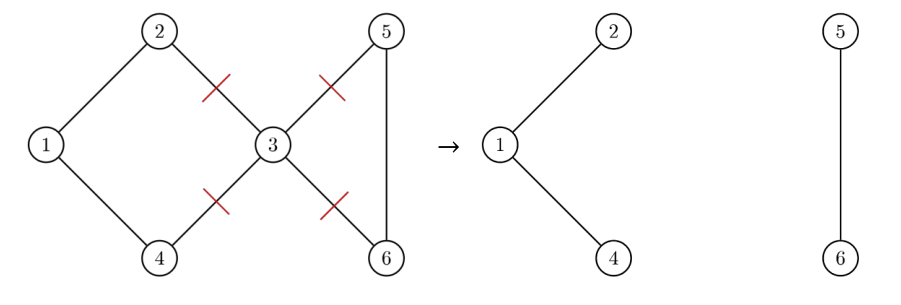
\includegraphics[scale=0.3]{15.png}
\end{figure}

В данном графе вершина 3 является \textit{шарниром}.

\begin{definition}
    \textit{Мостом} в графе называется ребро, удаление которого
    приводит к увеличению числа компонент связности.
\end{definition}

\begin{figure}[h]
    \centering
    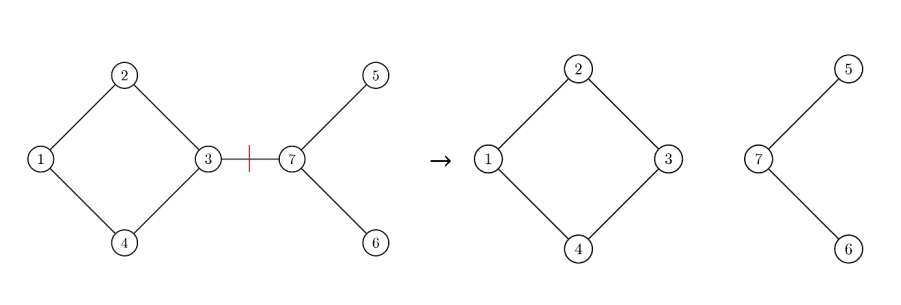
\includegraphics[scale=0.35]{15_2.png}
\end{figure}

Ребро $(3,7)$ является \textit{мостом}.

\newpage
\textbf{Алгоритм нахождения мостов графа:}
\begin{enumerate}[left=0.0em, labelsep=1em, topsep=0.0em, itemsep=0pt, parsep=0.5em]
    \item Проводим поиск в графе в глубину. При появлении новой вершины
    записываем ее в последовательность $L$. При прохождении ребра $(u,v)$ делаем
    ребро ориентированным, а именно, запрещаем прохождение при втором
    поиске в глубину по этому ребру в направлении от вершины $u$ к вершине $v$.
    \item Проводим второй поиск в глубину с учетом ориентированности ребер.
    (если по ребру не проходили, то можно по нему идти в любую сторону).
    Вершины, из которых начинаем обход, берем в порядке из
    последовательности $L$, полученной в шаге 1. Вершинам из одной компоненты
    приписываем один цвет.
    \item Ищем ребра графа, вершины которого раскрашены в разный цвет. Это
    и будут мосты.
\end{enumerate}

Пример алгоритма на графе:
\begin{figure}[h]
    \centering
    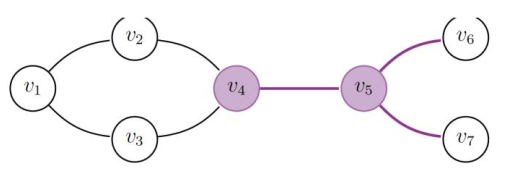
\includegraphics[scale=0.35]{15_3.png}
\end{figure}
\begin{figure}[h]
    \centering
    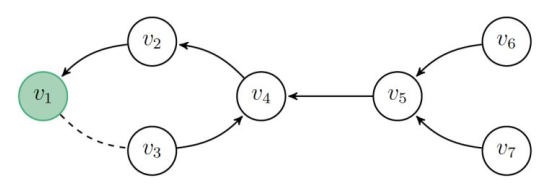
\includegraphics[scale=0.35]{15_4.png}
\end{figure}
\begin{figure}[h]
    \centering
    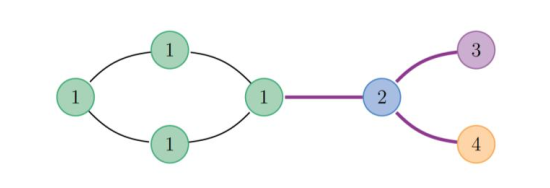
\includegraphics[scale=0.35]{15_5.png}
\end{figure}

Находим ребра, вершины которых раскрашены в разный цвет -- это и будут
мосты: $(4,5), (5,6), (5,7)$.